\documentclass[11pt,xcolor={dvipsnames},hyperref={pdftex,pdfpagemode=UseNone,hidelinks,pdfdisplaydoctitle=true},usepdftitle=false]{beamer}
\usepackage{customtikz}
\usepackage{presentation}
\usepackage{kotex}
\usepackage{amsmath}
\usepackage{amsthm}
\usepackage{amsfonts}
\usepackage{graphicx}
\usepackage{hyperref}
\usepackage{algorithm2e}
\usepackage{subcaption}
\usepackage{lscape}
\usepackage[table,xcdraw]{xcolor} % For coloring table cells and drawing colors
\usepackage{array}
\usepackage{colortbl}
\usepackage{makecell} % For easy multi-line cells

% Enter title of presentation PDF:
\hypersetup{pdftitle={Minimalist LaTeX Template for Academic Presentations}}
% Enter link to PDF file with figures:
\newcommand{\resStk}{figs/result_stk.pdf}
\newcommand{\resMario}{figs/mario-result.pdf}

% https://shuijing725.github.io/files/20190926_DAgger.pdf  More references

\begin{document}
% Enter presentation title:
\title{A Reduction of Imitation Learning and Structured Prediction \\ to No-Regret Online Learning (DAgger)}
\information
% 
[http://www.yisongyue.com/courses/cs159/lectures/imitation-learning-3.pdf]
% 
{임건호}
% 
{2024.06.21}

\frame{\titlepage}

% Fill out content of presentation:
\section{Introduction}

\begin{frame}
\frametitle{논문이 풀고자 하는 문제 {\small (제목을 이해해보자)}}

Imitation Learning when expert policy exists!

\begin{itemize}
\item Reduction: Imitation Learning 문제를 근사하여 \\ 다른 문제로 바꾸는 것
\item Regret: 매 순간순간 최선의 선택을 하는 것 \\ {\footnotesize (cf. 헛된 일(Exploration)을 하면 후회 함)}
\item Online Learning: 모델이 전체 데이터를 보지 않고, \\ 순차적으로 데이터를 받아들이는 학습 방법
\end{itemize}


% \begin{figure}
%     \centering
%     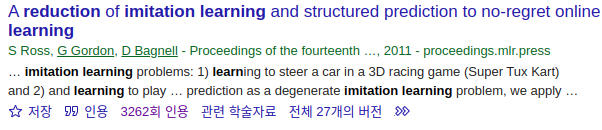
\includegraphics[width=\textwidth]{figs/citation.png}
% \end{figure}

\vspace{-10mm}

\begin{figure}
    \centering
    \begin{equation}
        \frac{1}{N} \sum_{i=1}^N \ell_i(\pi_i) - \min_{\pi \in \Pi} \frac{1}{N} \sum_{i=1}^N \ell_i(\pi)
    \end{equation}
    \vspace{-5mm}
    \caption{Regret 정의}
\end{figure}
\end{frame}

\begin{frame}
\frametitle{그래서, 어디에 쓸모가 있을까?}

네트워크 구조를 바꾸면서 이전 네트워크의 knowledge를 \\ 
유지하고 싶을 때

\begin{itemize}
    \item {\href{https://www.youtube.com/watch?v=2rQAW-8gQQk}{Catch \& Carry (영상)}}
    \item {\href{https://www.youtube.com/watch?v=uCjQXowIChU}{Progressive RL (영상)}}
    \item PULSE, Neural Categorical Prior(NCP)
    \item Offline RL이 왜 잘 안되는지 이해할 수 있음
\end{itemize}

\begin{figure}
    \centering
    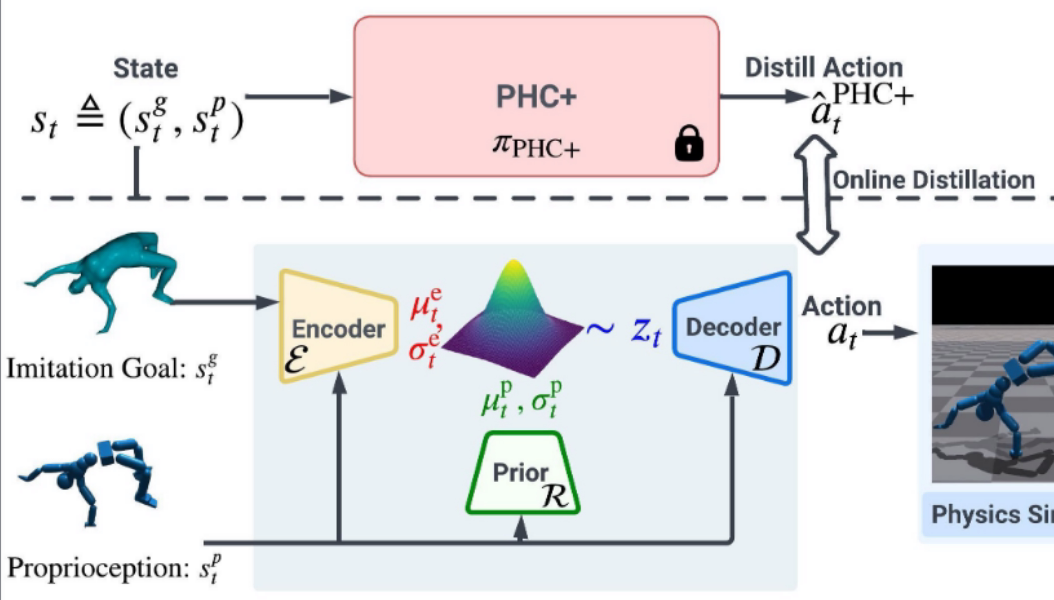
\includegraphics[width=0.6\textwidth]{figs/PULSE.png}
    \caption{PULSE 학습 과정}
\end{figure}

\end{frame}

\section{Background}

\begin{frame}
\frametitle{Na\"{i}ve Approach of Imitation Learning}
\begin{defn}[{Supervised Learning}]
    {\small $\pi$와 $\pi^*$이 \, 동일한 \, state($s \sim d_{\pi^*}$)에서 활동한다고 가정하면,}
    \begin{equation}
        \hat{\pi}_{sup} = \argmin_{\pi \in \Pi}{\mathbb{E}_{s \sim d_{\pi^*}}[\ell(s,\pi)]}
    \end{equation}
\end{defn}

\vspace{-5mm}
{\footnotesize 학습된 $\hat{\pi}$는 $\pi^*$와 학습 오차로 인해 state의 분포가 다르고, \\ 벗어난 경로를 회복하는 action을 보지 못하여 trajectory 발산}

\begin{figure}
    \centering
    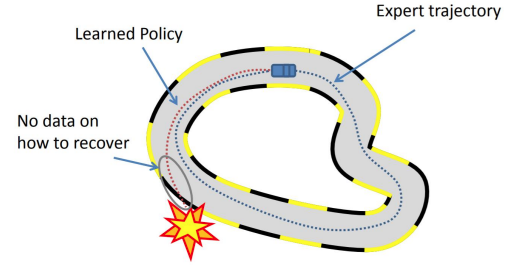
\includegraphics[width=0.7\textwidth]{figs/path.png}
\end{figure}
\end{frame}

\begin{frame}
\frametitle{Notations}
\begin{itemize}
    \item $T$ the task horizon
    \item $d^t_\pi$ \, $t$ 시점의 state의 분포
    \item $d_\pi = \frac{1}{T} \sum_{t=1}^T d^t_\pi$ \, states의 평균
    \item $C(s,a)$ cost
    \item $C_\pi(s) = \mathbb{E}_{a \sim \pi(s)}[C(s,a)]$ \, C의 정의에서 $\pi$ 고정
    \item $C$ is bounded in $[0,1]$
    \item $J(\pi) = \sum_{t=1}^T \mathbb{E}_{s \sim d^t_\pi}[C_\pi(s)] = T \mathbb{E}_{s \sim d_\pi}[C_\pi(s)]$ \\ $\pi$에 의한 state에 대한 전체 cost
    \item $\ell$ \, surrogate loss, C와 같을수도, 다를수도 있음 \\
    $\Rightarrow$ {\small $\hat{\pi}_{sup}$은 $\pi^*$의 state에 대해 $\ell$을 최소화하는 $\pi$}
\end{itemize}
\end{frame}

\begin{frame}
\frametitle{Na\"{i}ve Approach}
\begin{theorem}[{Na\"{i}ve는 Quadratic Loss}]
    $\ell(s,\pi)$ loss of $\pi$ with respect to $\pi^*$ \\
    $\mathbb{E}_{s \sim d_{\pi^*}}[\ell(s,\pi)] = \epsilon$ \, (학습 과정에서 발생한 최대 오차)
    \begin{equation}
        J(\pi) \leq J(\pi^*) + T^2 \epsilon
    \end{equation}
    Horizon 길이의 제곱에 비례하는 오차가 발생 (tight bound)
\end{theorem}

\begin{spacedProof}
    Let, $\ell(s, \hat{\pi})=I(\hat{\pi}(s)\neq\pi^*(s))$ \, $\hat{\pi}$의 실수(mistake)에 대한 0-1 오차 \\
    확률 \(p_t\): \, \(\pi\)가 첫 \(t\)-step 동안 \(\pi^*\)에 대해 실수를 하지 않음 \\
    \(d_t\): \, $\hat{\pi}$이 실수를 하지 않았을 때 state의 분포 \\
\end{spacedProof}
\end{frame} 

\begin{frame}
\begin{spacedProof}[cont'd]
    \(d_t'\): \, $\hat{\pi}$이 적어도 한번 이상 실수 했지만, \(\pi^*\)를 따라갈 때 분포 \\
    \(\pi\)가 \(\pi^*\)을 따라가면, 실수를 하거나, 하지 않으므로, \\
    $\textbf{정리하면, \quad} d^{t}_{\pi^*} = p_t d_t + (1 - p_{t-1}) d_t'$ \\

    실수를 할때 cost의 상한은 1, 실수를 하지 않으면 \(\mathbb{E}_{s \sim d_t^{\pi}} (C_t^\pi (s))\)
    \[
    \textbf{따라서, \quad} J(\pi) \leq \sum_{t=1}^T [p_{t - 1} \mathbb{E}_{s \sim d_t^{\pi}} (C_t^\pi (s)) + (1 - p_{t-1})].
    \]

    Let, $\epsilon_i = \mathbb{E}_{s \sim d^{i}_{\pi^*}}[\ell(s, \hat{\pi})] \text{ for } i = 1, 2, \ldots, T$ \\ 
    $\pi^*$의 state에 대한 $\hat{\pi}$의 i 시점에서 오차 \\
    ($\ell$의 정의에 의해 $\hat{\pi}$을 따라갈 때 t 시점에서 실수할 확률과 같음) \\
\end{spacedProof}    
\end{frame}

\begin{frame}
\begin{proof}[cont'd]
    \begin{spacing}{1.5}
    \(e_t\) / \(e_t'\): \, state \(d_t\) / \(d_t'\)에서 \(\pi\)가 실수할 확률 ($\epsilon_i$ 와 다르다) \\
    t 시점에 $\pi$는 실수를 하거나, 하지 않으므로,
    \[
    \mathbb{E}_{s \sim d_t^{\pi}} (C_t^\pi (s)) \leq \mathbb{E}_{s \sim d_t^{\pi}} (C_t^* (s)) + \epsilon_t,
    \] \\ 
    또한, $\epsilon_t = p_{t - 1} e_t + (1 - p_{t-1}) e_t' \quad {\rightarrow} \quad p_{t - 1} e_t \leq \epsilon_t$ \\
    추가로, \(p_t = (1 - e_t)p_{t - 1}\) \\
    그런데, 앞선 $d_t^{\pi^*}$ 계산식에 의하면, \\
    \(J(\pi^*) = \sum_{t=1}^T [p_{t - 1} \mathbb{E}_{s \sim d_t^{\pi}} (C_t^* (s)) + (1 - p_{t-1}) \mathbb{E}_{s \sim d_t^{\pi}} (C_t^* (s))]\) 이고
    \[ \Longrightarrow  
    \sum_{t=1}^T p_t - 1 \mathbb{E}_{s \sim d_t^{\pi}} (C_t^* (s)) \leq J(\pi^*).
    \]
    \end{spacing}
\end{proof}    
\end{frame}

\begin{frame}
\begin{spacedProof}[cont'd]
    정리하면:
    \begin{align}
        J(\pi) &\leq \sum_{t=1}^T \left[ p_{t - 1} \mathbb{E}_{s \sim d_t^{\pi}} (C_t^\pi (s)) + (1 - p_{t-1}) \right] \nonumber \\
        &\leq J(\pi^*) + \sum_{t=1}^T \sum_{i=1}^t \epsilon_i \nonumber \\
        &\leq J(\pi^*) + T \sum_{t=1}^T \epsilon_t = J(\pi^*) + T^2 \epsilon.
    \end{align}\end{spacedProof}    
    (\(\epsilon = \frac{1}{T} \sum_{i=1}^T \epsilon_i\): \, 학습 오차의 평균) \\

    \vspace{7mm}

    이 증명은 논문에 포함된 6개 증명 중 하나로서 \\ 가장 쉬운(!) 증명이다.

\end{frame}

\section{Previous Work}

\begin{frame}
\heading{Previous Works}
\end{frame}

\subsection*{Forward Training}
\begin{frame}
\frametitle{Forward Training}
\begin{algorithm}[H]
    \SetAlgoLined
    \KwData{$\pi_1^0, \ldots, \pi_T^0$ to query and execute $\pi^*$.}
    \For{$i = 1$ to $T$}{
        Sample $T$-step trajectories by following $\pi^{i-1}$\;
        Get dataset $\mathcal{D} = \{(s_i, \pi^*(s_i))\}$ of states, actions taken by expert at step $i$\;
        Train classifier $\pi_i^i = \arg\min_{\pi \in \Pi} \mathbb{E}_{s \sim \mathcal{D}} (\epsilon_{\pi}(s))$\;
        $\pi_j^i = \pi_j^{i-1}$ for all $j \ne i$\;
    }
    \Return $\pi_1^T, \ldots, \pi_T^T$\;
\end{algorithm}
\end{frame}


\begin{frame}
\frametitle{Forward Training}
i가 작을때는, $s~\pi^*$ 위주로 학습하고, \\ 
i가 커질수록 $\pi^{i-1}$에 의해 학습된 데이터를 이용하여 학습    

\vspace{5mm}

\begin{itemize}
    \item $J(\pi) \leq  J(\pi^*) + u T \epsilon$ \, (u는 대개 상수, T에 선형)
    \item $\pi$에 의한 오차를 $\pi^*$으로 복구하는 방법 학습
    \item T개의 classifier를 학습하므로, T가 큰 경우에 비효율적
    \item Motion VAE에서 Autoregressive하게 훈련하는 것은 \\ $\pi_j^i = \pi_j^{i-1}$ 조건을 무시한 것으로 볼 수 있음
\end{itemize}
\end{frame}
    
\subsection*{SMILe}
\begin{frame}
\frametitle{Stochastic Mixing Iterative Learning (SMILe)}

이전 policy를 stochastic하게 혼합하여 학습

\vspace{3mm}

\begin{algorithm}[H]
    \SetAlgoLined
    \KwData{$\pi^0$ expert $\pi^*$로 초기화}
    \For{$i = 1$ to $N$}{
        Execute $\pi^{i-1}$ to get $\mathcal{D} = \{(s, \pi^*(s))\}$\ \\
        Train classifier $\hat{\pi}^i = \arg\min_{\pi \in \Pi} \mathbb{E}_{s \sim \mathcal{D}}(\epsilon_{\pi}(s))$\ \\
        $\pi^i = (1-\alpha)^i \pi^* + \alpha \sum_{j=1}^i (1-\alpha)^{i-j} \hat{\pi}^j$\ \\
    }
    Remove expert queries: $\tilde{\pi}^N = \frac{\pi^N - (1-\alpha)^N \pi^*}{1 - (1-\alpha)^N}$\ \quad (정규화) \\ 
    \Return $\tilde{\pi}^N$\ 
\end{algorithm}

\vspace{2mm}

\begin{itemize}
    \item Normalize하여 결국 $\pi_0$ 제거 
    \item T에 선형인 오차 bound
    \item 임의의 N을 사용할 수 있어 feasible한 알고리즘
\end{itemize}
\end{frame}

\section{DAgger}

\begin{frame}
\heading{Can we do better?}
\end{frame}

\subsection*{Property}
\begin{frame}
\frametitle{DAgger algorithm}

$\hat{\pi}$가 실수할 수 있는 경로를 모두 합집합(Aggregate)한 \\ 데이터셋($\mathcal{D}$)을 이용하여 학습

\vspace{3mm}

\begin{algorithm}[H]
    \SetAlgoLined
    \KwData{Initial dataset $\mathcal{D} \leftarrow \emptyset$.}
    \KwData{Initial policy $\hat{\pi}_1 \in \Pi$. \quad (말그대로 임의의 policy)}
    \For{$i = 1$ \KwTo $N$}{
        Let $\pi_i = \beta_i \pi^* + (1-\beta_i) \hat{\pi}_{i}$\;
        Sample $T$-step trajectories using $\pi_i$\;
        Get dataset $\mathcal{D}_i = \{ (s, \pi^*(s)) \}$ of visited states by $\pi_i$\;
        Aggregate datasets: $\mathcal{D} \leftarrow \mathcal{D} \cup \mathcal{D}_i$\;
        Train classifier $\hat{\pi}_{i+1}$ on $\mathcal{D}$\;
    }
    \KwResult{Best $\hat{\pi}_i$ on validation}
    \end{algorithm}

\end{frame}    

\begin{frame}
\frametitle{DAgger algorithm}
\begin{itemize}
    \item 이전(\textit{Forward, SMILe})은 $\mathcal{D}$를 한번 사용하고 버렸지만, \\ DAgger는 계속해서 사용
    \item 일반적으로 $\beta_i = p^{i-1}$로 설정 ($\pi_1$을 임의로 설정)
    \item No Regret {\scriptsize (Asymptotic Optimal, Stable)} \\
    $\Leftrightarrow$ Immediate/Expected Loss minimization
\end{itemize}

\begin{equation}
    \frac{1}{N} \sum_{i=1}^N \ell_i(\pi_i) - \min_{\pi \in \Pi} \frac{1}{N} \sum_{i=1}^N \ell_i(\pi) \leq \gamma_N \lim_{N \to \infty} 0
\end{equation}
\end{frame}

\begin{frame}
    \frametitle{DAgger is No Regret}
    \begin{theorem}[Follow the Leader(FTL)]
        $\pi_N$ = argmin $\sum_{i=1}^{N-1} \ell_i(\pi)$ \\
    \end{theorem}
    
    FTL is no regret algorithm (다른 paper에서 증명) \\
    DAgger은 전체 데이터셋을 optimize하여 학습하므로, \\
    FTL을 따르면서 학습하므로 No Regret 성질을 가짐
\end{frame}    

\subsection*{Expert 수렴}
\begin{frame}
\frametitle{DAgger algorithm은 Expert에 수렴 (Proof)}
Let $\epsilon_N = \min_{\pi \in \Pi} \frac{1}{N} \sum_{i=1}^N \mathbb{E}_{s \sim d_{\pi_i}}[ \ell(s,\pi) ]$ \\
the true loss of the best policy in hindsight. \\
(돌이켜 봤을 때 가장 좋은 policy(student+expert mix)의 loss)

\begin{theorem}[Student loss는 $\epsilon_N$에 수렴]
    For \textsc{DAgger}, if $N$ is $\tilde{O}(T)$, \: $\exists \hat{\pi} \in \hat{\pi}_{1:N}$ s.t. \\
    $\mathbb{E}_{s \sim d_{\hat{\pi}}}[ \ell(s,\hat{\pi}) ] \leq \epsilon_N + O(1/T)$

    {\small ($\tilde{O}(T)$는 \: $\exists k$ s.t. $N = O(T \cdot log^k(T))$, \: polylogarithmic in $T$)}
\end{theorem}

\begin{theorem}[Total Cost역시 수렴]
    if $N$ is $\tilde{O}(uT)$, \: $\exists \hat{\pi} \in \hat{\pi}_{1:N}$ s.t. \\
    $J(\hat{\pi}) \leq J(\pi^*) + uT\epsilon_N + O(1)$.
\end{theorem} 
\end{frame}


\begin{frame}
\frametitle{DAgger algorithm - Finite Sample (Proof)}
Trajectory를 모두 sample 할 수 없음 (finite sample, m) \\
$\Rightarrow$ $\hat{\epsilon}_N$에 대해 앞선 부등식 증명 가능

\vspace{10mm}

앞선 부등식을 만족하는 $\hat{\pi}$은 확률적으로 존재

\end{frame}
    
\subsection*{Optimality}

\begin{frame}
\frametitle{DAgger algorithm - Online Learning (Proof)}
\textsc{DAgger}의 No Regret 성질로 more tight upper bound \\
$\Rightarrow$ $\pi_{1:N}$ 중에 가장 좋은 policy와 비슷한 성능

\begin{theorem}[{State 분포의 차이는 Bounded}]
    $||d_{\pi_i} - d_{\hat{\pi}_i}||_1 \leq 2 T \beta_i$
\end{theorem}    

\begin{theorem}[{DAgger Upper Bound}]
    $\exists \hat{\pi} \in \hat{\pi}_{1:N}$ s.t. \\
    $\mathbb{E}_{s \sim d_{\hat{\pi}}}[ \ell(s,\hat{\pi}) ] \leq \epsilon_N + \gamma_N + \frac{2 \ell_{\max}}{N} [n_\beta + T \sum_{i=n_\beta+1}^N \beta_i]$, \\
    ($\gamma_N$ = average regret of $\hat{\pi}_{1:N}$)
\end{theorem}    

$N \to \infty$일때, 두번째, 세번째 항은 0으로 수렴 \\
Finite Sample에서도 $\hat{\pi}$는 $\epsilon_N$에 수렴

\end{frame}

\section*{Comparison}

\begin{frame}
\frametitle{Visualize}
\begin{figure}[ht]
    \centering
    \begin{subfigure}[b]{0.3\textwidth}
        \centering
        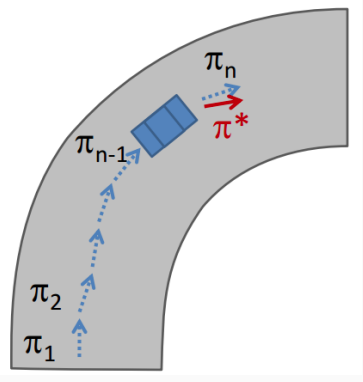
\includegraphics[width=\textwidth]{figs/forward.png}
        \caption{{\small Forward Training}}
        \label{fig:forward}
    \end{subfigure}
    \begin{subfigure}[b]{0.3\textwidth}
        \centering
        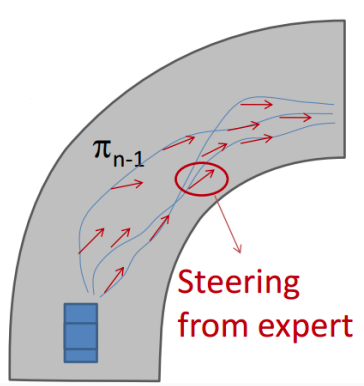
\includegraphics[width=\textwidth]{figs/smile.png}
        \caption{{\small SMILe}}
        \label{fig:smile}
    \end{subfigure}
    
    \begin{subfigure}[b]{0.3\textwidth}
        \centering
        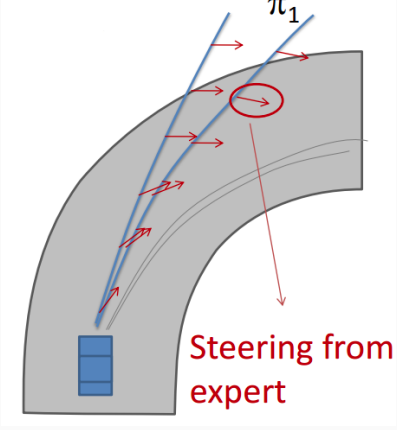
\includegraphics[width=\textwidth]{figs/dagger1.png}
        \caption{{\small Initial DAgger}}
        \label{fig:dagger1}
    \end{subfigure}
    \begin{subfigure}[b]{0.3\textwidth}
        \centering
        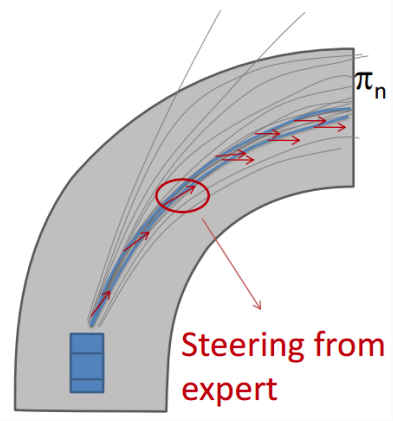
\includegraphics[width=\textwidth]{figs/daggern.png}
        \caption{{\small Last DAgger}}
        \label{fig:daggern}
    \end{subfigure}\end{figure}
\end{frame}

\section*{Result}

\begin{frame}
\heading{Result}
\end{frame}

\begin{frame}
\frametitle{Tasks}

Imitation Learning 문제와 라벨링 문제

\vspace{5mm}

\begin{itemize}
    \item Super Tux Kart: \quad (Image) $\rightarrow$ (Joystick)
    \item 슈퍼 마리오: \quad (Image) $\rightarrow$ (4 방향)
    \item Handwriting 인식: \quad (Image) $\rightarrow$ (Class)
\end{itemize}
\begin{figure}
    \setcounter{subfigure}{0}
    \centering
    \begin{subfigure}[b]{0.3\textwidth}
        \centering
        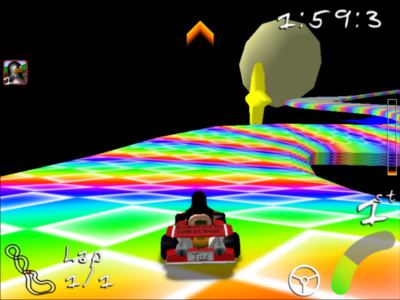
\includegraphics[width=\textwidth]{figs/stk.png}
        \caption{Super Tux Kart}
        \label{fig:stk}
    \end{subfigure}
    \begin{subfigure}[b]{0.3\textwidth}
        \centering
        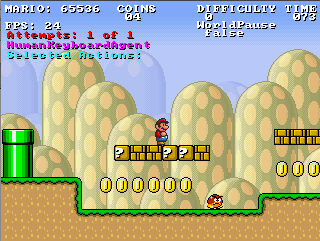
\includegraphics[width=\textwidth]{figs/mario.png}
        \caption{Super Mario}
        \label{fig:mario}
    \end{subfigure}
\end{figure}
\end{frame}

\begin{frame}
\frametitle{Results}

DAgger(파란색)가 다른 방법보다 더 나은 성능을 보임

\begin{figure}
    \centering
    \captionsetup[subfigure]{position=above, justification=centering}
    \begin{subfigure}{0.45\textwidth}
        \centering
        \includegraphics[width=\textwidth]{\resStk}
        \vspace{-15mm}
        \caption{Super Tux Kart \\ (Falls Per Lap)}
        \label{fig:resStk}
    \end{subfigure}
    \hfill
    \begin{subfigure}{0.45\textwidth}
        \centering
        \includegraphics[width=\textwidth]{\resMario}
        \vspace{-15mm}
        \caption{Super Mario \\ (Travelled Stage)}
        \label{fig:resMario}
    \end{subfigure}
    \label{fig:results}
\end{figure}

\end{frame}

\section*{Further Works}

\begin{frame}
\frametitle{AggreVaTe (RL version)}

{\small Current Cost 뿐만 아니라 Future Cost까지 고려한 학습 (Cost-to-go)}

\vspace{5mm}

\begin{algorithm}[H]
    \small
    \SetAlgoLined
    \KwData{Initialize $\mathcal{D} \leftarrow \emptyset$, $\hat{\pi}_1$ to any policy in $\Pi$.}
    \For{$i = 1$ \KwTo $N$}{
        Let $\pi_i = \beta_i \pi^* + (1 - \beta_i) \hat{\pi}_i$
        \For{$j = 1$ \KwTo $m$}{
            Sample $t \in \{1, 2, \ldots, T\}$\;
            Start new trajectory from initial state distribution\;
            Execute $\pi_i$ up to time $t - 1$\;
            Exploration action $a_t$ \;
            Execute expert from $t + 1$ to $T$\;
            Estimate of cost-to-go $\hat{Q}$ from $t$\;
        }
        Dataset $\mathcal{D}_i = \{(s, t, a, \hat{Q})\}$ \quad (이후 Dagger과 동일) \;
    }
    \Return best $\hat{\pi}_i$ on validation.
    \end{algorithm}

\end{frame}

\section*{Application}

\begin{frame}
    \heading{By the way, \\ how we handled the problem of \\ Imitation Learning?}
\end{frame}


\begin{frame}
\frametitle{GAIL \\ (Generative Adversarial Imitation Learning)}

AMP, ASE, PHC... 등이 사용하는 방법으로서, \\
GAN의 reward를 통해 expert trajectory로 guide

\vspace{5mm}

문제
\begin{enumerate}
\item RL을 사용하여야 함
\item GAN의 mode-collapse로 인해 diversity $\downarrow$ 
\end{enumerate}

\vspace{5mm}

$\Longrightarrow$ GAIL은 dataset만 가지고 있을 때, \\ 
\quad $\pi^*$를 생성하는 문제에 대한 방법론임 \\
$\therefore$ expert를 가지고 있을 때에는 굳이 사용할 필요 없음

\end{frame}


\begin{frame}
\frametitle{Supervised Learning}

MotionVAE, ControlVAE 등이 사용하는 방법으로서, \\
autoregressive하게 네트워크의 출력을 입력으로 주어 \\ 
그 결과가 dataset을 따라가게 gradient 부여

\vspace{5mm}

$\Longrightarrow$ DAgger은 $\pi^*$를 가지고 있을 때  \\ 
Supervised Learning을 잘 하기 위한 방법 \\
(이렇게 할 일이 있을까?)

\end{frame}

% \begin{frame}
% \frametitle{Expert를 가지고 있을 때에는?}
% \begin{table}
%     \centering
%     \begin{tabular}{|>{\small}l|>{\small}l|>{\small}l|}
%         \hline
%         \rowcolor{lightgray} % Apply background color to the header row
%         & \textbf{ScaDiver} & \textbf{ASE} \\
%         \hline
%         \makecell{\textbf{Skill}\\\textbf{Combination}} & MoE & \makecell{Conditioned\\Network(z)} \\
%         \hline
%         \textbf{Control} & Gating Network & High Level Policy \\
%         \hline
%     \end{tabular}
% \end{table}

% \vspace{5mm}

% 기존의 방법은, Control Task에서 사용하는 state가 \\
% Low Level Task에 넣어주는 state를 같게 유지하여야 하므로 유연하지 않음

% $\Longrightarrow$ 유연하게 State를 바꾸어 줄 필요가 있을까?

% \end{frame}


\begin{frame}
    \frametitle{Expert를 가지고 있을 때에는?}
    Distillation이라는 용어를 사용한 작업들

    \begin{table}
        \centering
        \begin{tabular}{|>{\small}l|>{\small}l|}
            \hline
            \rowcolor{lightgray} % Apply background color to the header row
            & \textbf{목적} \\
            \hline
            \textbf{Catch\&Carry} & Policy input: \: marker $\to$ Image \\
            \hline
            \textbf{Progressive} & Adapt Terrain \\
            \hline
            \textbf{NCP} & Posterior(future frame) $\to$ Prior(no future) \\
            \hline
            \textbf{PULSE} & Policy structure: \: MoE $\to$ VAE \\
            \hline
        \end{tabular}
    \end{table}    

    \begin{figure}
        \centering
        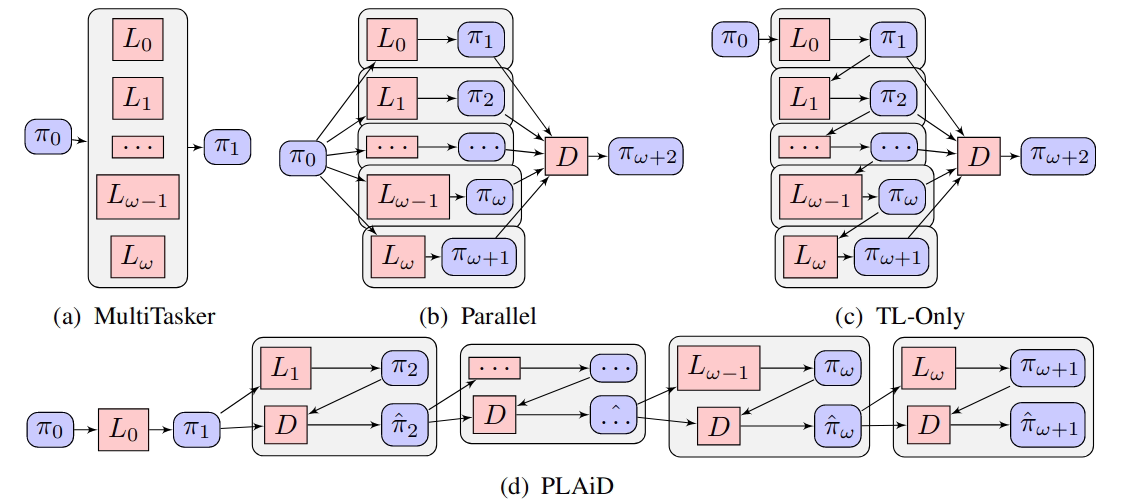
\includegraphics[width=0.8\textwidth]{figs/progressive.png}
        \caption{Progressive RL 학습 Curriculum {\footnotesize (D: distillation, L: learning)}}
    \end{figure}    
\end{frame}

\begin{frame}
\frametitle{나의 연구에 어떻게 적용할 수 있을까?}
목적: 두 캐릭터에 대해 캡쳐된 모션을 사용하여 \\ 
1. N 캐릭터가 상호작용 하는 모션 생성 혹은 \\
2. 상대 캐릭터 행동에 적절한 반응을 하는 모션 생성

\vspace{5mm}

현재 구상하는 구조

\begin{figure}
\centering
\begin{tikzpicture}[
    scale=0.8,
    transform shape,
        anchor=west,
        disc/.style={
            rectangle,
            draw=orange, 
            thick, 
        },
        ]

    \def\varDistx{0.5cm}
    \def\varDisty{0.8cm}
    \def\blkDist{0.4cm}

    % % Nodes
    \node[enc] (posterior) {\rotatebox{90}{$
        \begin{array}{c} 
            Encoder
        \end{array}
    $}};

    % \node[anchor=south, disc] (discrim) at ([yshift=\blkDist * 2]posterior.west) {$
    %     \begin{array}{c} 
    %         Discriminator \\ (naive \, state \: or \: IG)
    %     \end{array}    
    % $};
    
    \node[anchor=east] (t3) at ([xshift=-\varDistx]posterior.south){$s_{adv}(t-1)$};

    \node[] (z) at ([xshift=\blkDist]posterior.north) {$z$};
    
    \node[dec, anchor=north] (decoder) at ([xshift=\blkDist]z.east) {\rotatebox{-90}{$Decoder$}};
    
    \node[scale=1.4] (t4) at ([xshift=\varDistx]decoder.south) {$\hat{s}_{self}(t)$};
    \node[anchor=north] (t5) at ([yshift=-1cm]decoder.west) {$s_{self}(t-1)$};
    
    % % Arrows
    \draw[line] (t3) -- (posterior.south);
    % \draw[line] (discrim) -- (posterior.west) node [right, yshift=0.5cm] {Loss};
    \draw[line] (posterior) -- (z);

    % Calculate midpoint of the line from decoder.west to t5.north
    \coordinate (decLineMid) at ($(decoder.west)!0.8!(t5.north)$);
    \draw[line] (z) -- (decoder);
    \draw[line] (decoder) -- (t4);
    \draw[line] (t5) -- (decoder) node[] (decLine) {};
    \draw[line] (decLineMid) -| (posterior.east);    
    \end{tikzpicture}
\end{figure}

하나의 네트워크로 학습하면, 결과가 좋지 못하다. \\
Posterior collapse + 동작 6개 학습하는데 8시간 소요
\end{frame}

\begin{frame}
\frametitle{Abulation Study on PULSE}
PULSE에서는 $\pi_{PHC+}$를 distill 하여 $\pi_{PULSE}$를 학습 \\
Distill하지 않고, na$\ddot{i}$ve하게 학습한 결과

\begin{figure}
    \centering
    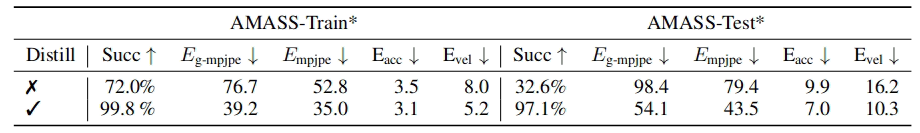
\includegraphics[width=\textwidth]{figs/distill_ab.png}
\end{figure}

(논문 주장) Latent와 Recon이 동시에 학습이 잘 안됨 \\
$\Rightarrow$ 나의 연구에도 시사하는 바가 있음, \\
Knowledge를 잘 전달하기 위해서는 어떻게 해야할까?

\end{frame}    

\begin{frame}
    \heading{Thank you}
\end{frame}

\lastslide

\end{document}